\section{Полносвязная нейронная сеть (Персептрон).}

\subsection{Модель нейрона МакКаллока-Питтса}

Рассмотрим модель нейрона МакКаллока-Питтса (1943) \cite{ModelMcCullochPitts}. Множество объектов $X$ (количество элементов множества $M$), множество ответов $Y$ (количество элементов множества $H_L$). Признаки объектов задаются вектором функций $\overrightarrow{f(x)} = [f_1(x), f_2(x), \dots, f_n(x)]^T$ таких, что $f_j: X \rightarrow \mathbb{R}$. Для объекта $x_m \in X$ с помощью этих функций определяется вектор вещественных признаков $\overrightarrow{x_m} = [x_m^1, x_m^2, \dots, x_m^n]^T$, где $x_m^j = f_j (x_m)$. Нейрон вычисляет функцию активации $\sigma$ от линейной комбинации вектора признаков $\overrightarrow{x_m}$ с весами $\overrightarrow{w}$. То есть выход нейрона $a(\overrightarrow{x_m}, \overrightarrow{w})$ вычисляется по формуле:
$$
a(\overrightarrow{x_m}, \overrightarrow{w}) = \sigma(\sum_{i = 1}^{n} x_m^i w_i - w_0) = \sigma (<\overrightarrow{x_m}, \overrightarrow{w}>)
$$
Математическая модель нейрона изображена на рисунке \ref{img:McCullochPittsModel}. Функцией активации $\sigma$ может быть любая непрерывная нелинейная функция. Нелинейность функции нужна, чтобы иметь возможность приблизить любую непрерывную функцию с желаемой точностью (теорема Горбаня, 1998). В формуле вектор признаков $\overrightarrow{x_m}$ дополнен элементом $-1$, который имеет вес $w_0$, что соответствует физической интерпретации нейрона. Нейрон $m$ получает на вход множество электрических сигналов $x_m^i$ по дендритам $i$. Каждый дендрит $i$ имеет свою толщину, и соответственно проводимость $w_i$. Чем выше проводимость $w_i$, тем больший вклад сигнала с данного дендрита в общую сумму. Нейрон суммирует сигналы с дендритов и если сумма выше порогового значения $w_0$, то он передаёт информацию дальше по аксону. Сигнал на выходе нейрона, то есть аксоне, определяется функцией активации $\sigma$.

\begin{figure}[h]
	\centering
	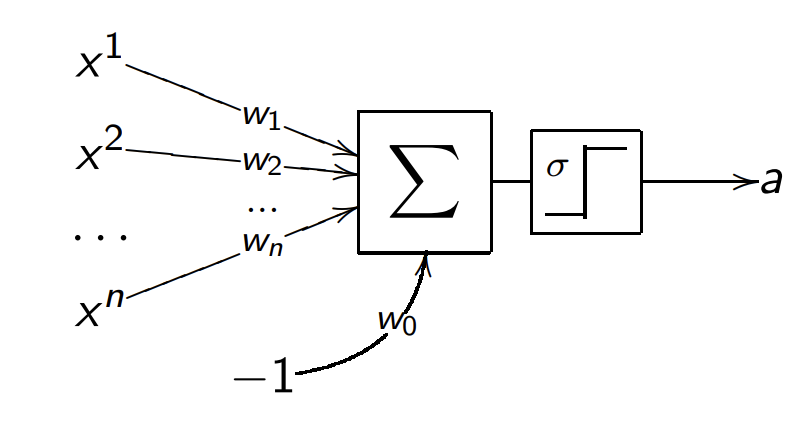
\includegraphics[width=0.4\linewidth]{chapters/neural/images/neuron1.png}
	\caption{Математическое описание модели нейрона МакКаллока-Питтса.}
	\label{img:McCullochPittsModel}
\end{figure}

\subsection{Реализация логических функций с помощью нейрона}

Рассмотрим применение описанного выше нейрона для реализации простейших логических функций.

\textbf{Логическая функция <<и>>}. Обозначение $\wedge$. На вход поступают признаки $x^1, x^2$, результат функции $a = x^1 \wedge x^2$. Нейронной реализацией будет $a = [x^1 + x^2 - \frac{3}{2} > 0]$, где функция активации $[x > 0]$ равна 1, если $x > 0$, и равна 0 в противном случае.

\begin{figure}[h]
	\centering
	\subfloat[Таблица истинности функции <<и>>]{
		\centering
		\begin{tabular}{|c|c|c|}
			\hline
			$x^1$ & $x^2$ & $a = x^1 \wedge x^2$ \\
			\hline
			0 & 0 & 0 \\
			0 & 1 & 0 \\
			1 & 0 & 0 \\
			1 & 1 & 1 \\
			\hline
		\end{tabular}
	}
	\hfill
	\subfloat[Модель нейрона, описывающего функцию <<и>>]{
		\centering
		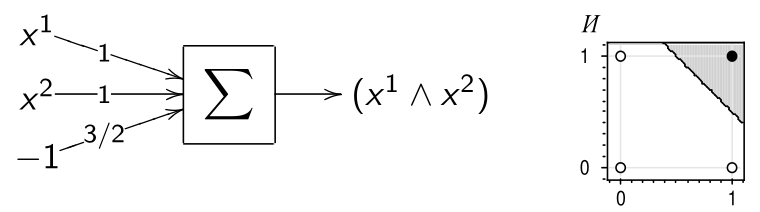
\includegraphics[width=0.45\linewidth]{chapters/neural/images/function_and.png}
	}
\end{figure}

\textbf{Логическая функция <<или>>}. Обозначение $\vee$. На вход поступают признаки $x^1, x^2$, результат функции $a = x^1 \vee x^2$. Нейронной реализацией будет $a = [x^1 + x^2 - \frac{1}{2} > 0]$, где функция активации $[x > 0]$ равна 1, если $x > 0$, и равна 0 в противном случае.

\begin{figure}[h]
	\centering
	\subfloat[Таблица истинности функции <<или>>]{
		\centering
		\begin{tabular}{|c|c|c|}
			\hline
			$x^1$ & $x^2$ & $a = x^1 \vee x^2$ \\
			\hline
			0 & 0 & 0 \\
			0 & 1 & 1 \\
			1 & 0 & 1 \\
			1 & 1 & 1 \\
			\hline
		\end{tabular}
	}
	\hfill
	\subfloat[Модель нейрона, описывающего функцию <<или>>]{
		\centering
		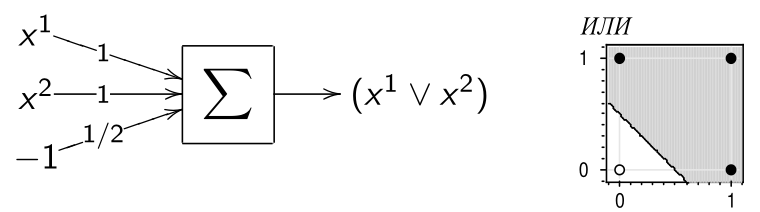
\includegraphics[width=0.45\linewidth]{chapters/neural/images/function_or.png}
	}
\end{figure}

\textbf{Задача 1.} Привести модель нейрона, описывающего логическую функцию <<не>> $\neg x^1$.

\textbf{Решение:}

$a = [-x^1 + 1/2 > 0]$

\newpage

\textbf{Логическая функция <<исключающее или>>}. Обозначение $\oplus$. Данная функция не реализуема с помощью одного нейрона. Но может быть реализована нейронной сетью $[n_1, n_2, n_3]$: $n_1 = (x^1 \vee x^2)$, $n_2 = (x^1 \wedge x^2)$, $n_3 = [n_1 - n_2 - \frac{1}{2} > 0]$.

\begin{figure}[h]
	\centering
	\subfloat[Таблица истинности функции <<исключающее или>>]{
		\centering
		\begin{tabular}{|c|c|c|}
			\hline
			$x^1$ & $x^2$ & $a = x^1 \oplus x^2$ \\
			\hline
			0 & 0 & 0 \\
			0 & 1 & 1 \\
			1 & 0 & 1 \\
			1 & 1 & 0 \\
			\hline
		\end{tabular}
	}
	\hfill
	\subfloat[Модель нейрона, описывающего функцию <<исключающее или>>]{
		\centering
		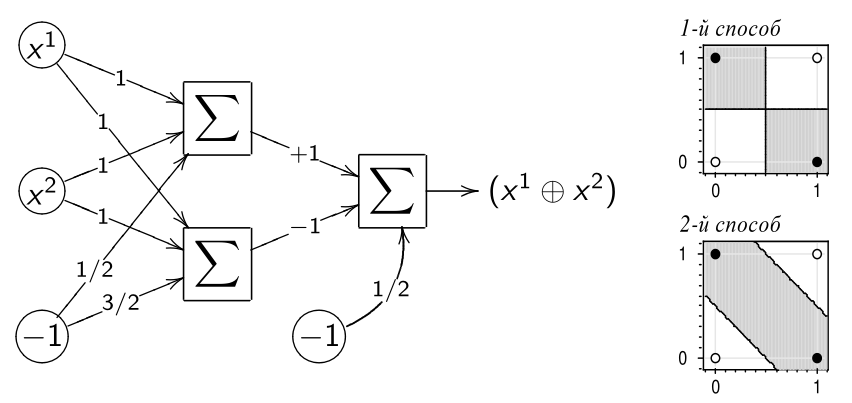
\includegraphics[width=0.45\linewidth]{chapters/neural/images/function_xor.png}
	}
\end{figure}

\textbf{Задача 2.} Привести модель нейронной сети, описывающей логическую функцию $f(x^1, x^2, x^3)$, заданную таблицей истинности: \\
\begin{figure}[h]
	\centering
	\begin{tabular}{|c|c|c|c|}
		\hline
		$x^1$ & $x^2$ & $x^3$ & $f(x^1, x^2, x^3)$ \\
		\hline
		0 & 0 & 0 & 0 \\
		0 & 0 & 1 & 1 \\
		0 & 1 & 0 & 0 \\
		0 & 1 & 1 & 0 \\
		
		1 & 0 & 0 & 1 \\
		1 & 0 & 1 & 1 \\
		1 & 1 & 0 & 0 \\
		1 & 1 & 1 & 1 \\
		\hline
	\end{tabular}
\end{figure}

\textbf{Решение:}

Используем ранее описанные нейроны <<и>> $\wedge$, <<или>> $\vee$, <<не>> $\neg$. Перепишем функцию, используя эти операции: $f = ((\neg x^1) \wedge ((\neg x^2) \wedge x^3)) \vee (x^1 \wedge ((\neg x^2) \vee x^3))$. Конструируем нейроны: $n_1 = \neg x^1$, $n_2 = \neg x^2$, $n_3 = n_2 \wedge x^3$, $n_4 = n_1 \wedge n_3$, $n_5 = n_2 \vee x^3$, $n_6 = x^1 \wedge n_5$, $n_7 = n_4 \vee n_6$. Итоговая многослойная нейронная сеть состоит из нейронов $n_1, n_2, \dots n_7$. Результат сети находится на выходе нейрона $n_7$.

\newpage

\subsection{Область применимости многослойных нейронных сетей}

Согласно \cite{VorontsovSite}
\begin{enumerate}
	\item Двухслойная сеть в ${0, 1}^n$ позволяет реализовать произвольную булеву функцию.
	
	\item Линейный нейрон в $\mathbb{R}^n$ отделяет полупространство признаков гиперплоскостью. Тогда двухслойная сеть позволяет отделить многогранную область, не обязательно выпуклую и связную.
	
	\item Согласно теоремы Горбаня (1998) с помощью линейных операций и одной нелинейной функции активации можно приблизить любую непрерывную функцию с любой желаемой точностью.
\end{enumerate}

\subsection{Полносвязная нейронная сеть}

Обобщением рассмотренной выше модели является полносвязная нейронная сеть (рис. \ref{img:full_net}). Сеть состоит из входного слоя (жёлтый цвет), скрытых слоёв (зелёный цвет), и выходного слоя (оранжевый цвет). Выход одного слоя, поступает на вход другого. Обозначим количество нейронов в слое $l$ за $H_l$, в каждом слое оно может быть разным, $l \in \{1, 2, \dots, L\}$. Всего $L$ слоёв. Вектор $x^l$ -- это выход $l$-ого слоя и вход $l+1$, если $l \neq L$, то есть $x^l$ -- не последний слой. $x^0$ -- это вход нейронной сети. Матрицы коэффициентов перехода между слоями обозначим за $W^l$. $W^l$ -- это матрица перехода между слоями $l-1$ и $l$.

\begin{figure}[h]
	\centering
	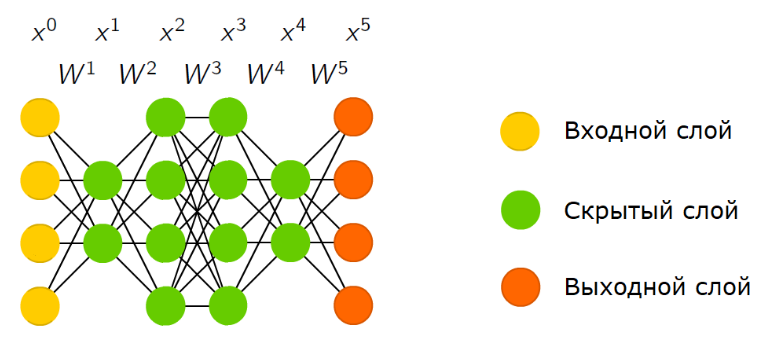
\includegraphics[width=0.6\linewidth]{chapters/neural/images/full_net.png}
	\caption{Полносвязная нейронная сеть.}
	\label{img:full_net}
\end{figure}

Задачей обучения нейронной сети является минимизация средних потерь на обучающей выборке $X$ ($|X| = M$):
$$
Q(\overrightarrow{W}, X) = \frac{1}{m} \sum\limits_{m = 1}^{M} \mathcal{L} (\overrightarrow{W}, x_m) \rightarrow \min_{\overrightarrow{W}}
$$

Пусть объект $x$ описывается вектором признаков $\overrightarrow{x} = [x_1, x_2, \dots, x_n]^T$. В задаче классификации множество ответов $Y$ состоит из $H_L$ элементов. Тогда последний слой нейронной сети $x^{L}$ должен содержать $H_L$ элементов. Нейронная сеть предсказывает ответ $k$, если на её выходе наблюдается вектор $x^L = [0, \dots 0, 1, 0, \dots 0]^T$, где единица стоит на $k$-ом месте. 

Функция потерь может быть, например, квадратичной. Для объекта $x$ функция потерь вычисляется по формуле $\mathcal{L} (\overrightarrow{W}^{(t)}, x) = \frac{1}{2} \sum\limits_{i = 1}^{H_L} (x^L_i ((\overrightarrow{W}^{(t)}, x) - y_i)^2$, где $\overrightarrow{y}$ -- вектор из всех нулей кроме единицы на месте порядкового правильного ответа из множества ответов.

Рассмотрим различные методы обучения полносвязной нейронной сети.

\subsection{Градиентный спуск}

\begin{enumerate}
	\item Выбираем какое-то начальное приближение вектора матриц перехода $\overrightarrow{W}^{(0)}$.
	
	\item Итерационный процесс:
		$$
		\overrightarrow{W}^{(t+1)} = \overrightarrow{W}^{(t)} - h \cdot \overrightarrow{\nabla} Q(\overrightarrow{W}^{(t)}, X)
		$$
		где $h$ -- градиентный шаг или темп обучения.
		
		Для рассмотренного ранее эмпирического риска:
		$$
		\overrightarrow{W}^{(t+1)} = \overrightarrow{W}^{(t)} - \frac{h}{m} \cdot \overrightarrow{\nabla} \sum\limits_{m = 1}^{M} \mathcal{L} (\overrightarrow{W}^{(t)}, x_m)
		$$
		
	\item Повторяем итерационный процесс, пока эмпирический риск $Q(\overrightarrow{W}^{(t)}, X)$ или вектор матриц перехода $\overrightarrow{W}$ не сойдутся. Критерий сходимости может быть абсолютным, то есть когда модуль разности значений на последовательных шагах итерационного процесса меньше какого-то значения $\varepsilon$. Например, для эмпирического риска:
	$$
	\left| Q^{(t + 1)} - Q^{(t)} \right| < \varepsilon
	$$
	Или может быть относительным, когда модуль отношения разности значений на последовательных шагах итерационного процесса к наименьшему, или наибольшему значению, или к первому меньше $\varepsilon$. Например, для эмпирического риска:
	$$
	\left| \frac{Q^{(t + 1)} - Q^{(t)}}{\min \{ Q^{(t + 1)}, Q^{(t)} \} } \right| < \varepsilon
	$$
	При этом для эмпирического риска и для вектора матриц перехода значение $\varepsilon$ может быть разным.
	
	Для вектора матриц перехода можно предложить следующий способ:
	$$
	\left|\left| \overrightarrow{W}^{(t+1)} - \overrightarrow{W}^{(t)} \right|\right|_1 = \sum\limits_{l = 1}^{L} \sum\limits_{m = 1}^{m_l} \sum\limits_{n = 1}^{n_l} |W^l_{mn}{}^{(t+1)} - W^l_{mn}{}^{(t)}|
	$$
	где вектор матрица перехода рассматривается как вектор всех её элементов, и применяется первая норма. Размерность матрицы $W^l$ равна $m_l \times n_l$. $W^l_{mn}{}^{(t)}$ -- это элемент в $m$-ой строке $n$-ого столбца матрицы перехода между слоями $l-1$ и $l$ на шаге $t$ итерационного процесса.
\end{enumerate}

Недостатком данного метода является низкая скорость сходимости. Для ускорения применяется метод стохастического градиентного спуска.

\subsection{Стохастический градиентный спуск}

В отличие от обычного градиентного спуска, в котором вектор матриц перехода изменяется пропорционально градиенту эмпирического риска для всех объектов, в стохастическом градиенте вектор матриц перехода изменяется пропорционально функции потерь для одного объекта.

Алгоритм стохастического градиента:

\begin{enumerate}
	\item Выбираем какое-то начальное приближение вектора матриц перехода $\overrightarrow{W}^{(0)}$. Вычисляем первое приближение эмпирического риска:
	$$
	Q^{(0)}(\overrightarrow{W}^{(0)}, X) = \frac{1}{m} \sum\limits_{m = 1}^{M} \mathcal{L} (\overrightarrow{W}^{(0)}, x_m)
	$$
	
	\item Итерационный процесс: \\
 	Выбираем какой-нибудь объект $x \in X$, например случайным образом или перебираем все элементы $X$ по порядку. Корректируем вектор матриц перехода:
	$$
	\overrightarrow{W}^{(t+1)} = \overrightarrow{W}^{(t)} - h \cdot \overrightarrow{\nabla} \mathcal{L} (\overrightarrow{W}^{(t)}, x)
	$$
	где $h$ -- темп обучения.
	
	Эмпирический риск оценивается по формуле:
	$$
	Q^{(t+1)}(\overrightarrow{W}^{(t+1)}, X) = \lambda \mathcal{L} (\overrightarrow{W}^{(t)}, x) + (1-\lambda)  Q^{(t)}(\overrightarrow{W}^{(t)}, X)
	$$
	где $\lambda$ -- темп забывания предыстории.
	
	Рассмотрим, откуда взялась эта оценка $Q^{(t+1)}$.
	
	Если $Q^{(t)}$ -- среднее арифметическое объектов $\varepsilon_i$, $i = 1, 2, \dots t$, то
	$$
	Q^{(t)} = \frac{1}{t} \varepsilon_t + \frac{1}{t} \varepsilon_{t-1} + \frac{1}{t} \varepsilon_{t-2} + \dots + \frac{1}{t} \varepsilon_{1}
	$$
	$$
	Q^{(t - 1)} = \frac{1}{t-1} \varepsilon_{t-1} + \frac{1}{t-1} \varepsilon_{t-2} + \dots + \frac{1}{t-1} \varepsilon_{1}
	$$
	$Q^{(t)}$ можно выразить через $Q^{(t-1)}$:
	$$
	Q^{(t)} = \frac{1}{t} \varepsilon_t + \frac{t-1}{t} Q^{(t-1)} = \frac{1}{t} \varepsilon_t + (1 - \frac{1}{t}) Q^{(t-1)}
	$$
	
	Если $Q^{(t)}$ -- экспоненциальное скользящее среднее с параметром $\lambda$, то
	$$
	Q^{(t)} = \lambda \varepsilon_t + \lambda (1-\lambda) \varepsilon_{t-1} + \lambda (1-\lambda)^2 \varepsilon_{t-2} + \dots + \lambda (1-\lambda)^{t-1} \varepsilon_{1}
	$$
	$$
	Q^{(t - 1)} = \lambda \varepsilon_{t-1} + \lambda (1-\lambda) \varepsilon_{t-2} + \lambda (1-\lambda)^2 \varepsilon_{t-3} + \dots + \lambda (1-\lambda)^{t-2} \varepsilon_{1}
	$$
	Или $Q^{(t)}$ через $Q^{(t-1)}$:
	$$
	Q^{(t)} = \lambda \varepsilon_t + (1 - \lambda) Q^{(t - 1)}
	$$
	
	Пусть теперь $\lambda \sim \frac{1}{t}$. Тогда $(1-\lambda)^{t-1} = (1 - \frac{1}{t})^{t-1}$. $\lim\limits_{t\rightarrow \infty} (1 - \frac{1}{t})^{t-1} = \frac{1}{e}$. По аналогии из радиотехники, где для экспоненциально убывающего сигнала характерное время затухания измеряется по уменьшению сигнала в $e$ раз, тогда характерное количество членов, когда происходит затухание / <<забывание>> предыдущей истории ряда равно $t$.
		
	\item Повторяем итерационный процесс, пока эмпирический риск $Q(\overrightarrow{W}^{(t)}, X)$ или вектор матриц перехода $\overrightarrow{W}$ не сойдутся.
\end{enumerate}

\subsection{Метод обратного распространения ошибок (BackProp).}

Для вычисления градиента функции потерь применяется метод обратного распространения ошибок. Для упрощения формулы индекс ${}^{(t)}$ будем опускать.
$$
\overrightarrow{\nabla} \mathcal{L} (\overrightarrow{W}, x) = \left[\frac{\partial}{\partial W^0}, \frac{\partial}{\partial W^\partial}, \dots, \frac{\partial}{\partial W^L}\right]^T \cdot \mathcal{L} (\overrightarrow{W}, x)
$$

Для рассмотренной ранее квадратичной функции потерь:
$$
\overrightarrow{\nabla} \mathcal{L} (\overrightarrow{W}, x) = \left[\frac{\partial}{\partial W^0}, \frac{\partial}{\partial W^\partial}, \dots, \frac{\partial}{\partial W^L}\right]^T \cdot \frac{1}{2} \sum\limits_{i = 1}^{H_L} (x^L_i ((\overrightarrow{W}, x) - y_i)
$$
То есть выход нейронной сети $\overrightarrow{x^L}$ является функцией от вектора матриц перехода $\overrightarrow{W}$.

Выведем формулу, по которой нейронная сеть вычисляет $\overrightarrow{x^L}$. На первом слое сети находится вектор $\overrightarrow{x^0}$, который через матрицу перехода $W^1$ и вектор функций активации $\overrightarrow{\sigma_1}$ преобразуется во вход второго слоя $x^1$:
$$
\overrightarrow{x^1} = \overrightarrow{\sigma_1} (W^1 \cdot \overrightarrow{x^0})
$$
Аналогично для последующих слоёв:
$$
\overrightarrow{x^2} = \overrightarrow{\sigma_2} (W^2 \cdot \overrightarrow{x^1}) = \overrightarrow{\sigma_2} (W^2 \cdot \overrightarrow{\sigma_1} (W^1 \cdot \overrightarrow{x^0}))
$$
$$
\overrightarrow{x^L} = \overrightarrow{\sigma_L}(W^L \cdot \overrightarrow{x^{L-1}}) = \overrightarrow{\sigma_L}(W^L \cdot \overrightarrow{\sigma_{L-1}} (W^{L-1} \cdot \overrightarrow{\sigma_{L-1}}( \dots ( W^2 \cdot \overrightarrow{\sigma_1} (W^1 \cdot \overrightarrow{x^0})) \dots ))
$$

Чтобы получить формулы для обратного распространения ошибок необходимо найти $\overrightarrow{\nabla} \mathcal{L}$, рассматривая $\overrightarrow{x^L}$ как функцию $\overrightarrow{x^L} (\overrightarrow{W})$.

\textbf{Задача 3.} Доказать рекуррентные формулы для метода обратного распространения ошибок в предположениях:
\begin{enumerate}
	\item Функция потерь квадратичная $\mathcal{L} (\overrightarrow{W}, x) = \frac{1}{2} \sum\limits_{i = 1}^{H_L} (x^L_i ((\overrightarrow{W}, x) - y_i)^2$.
	
	\item Первый нейрон в слое нейронной сети всегда -1, то есть $\forall i: x^i_0 = -1$. $H_l$ -- количество нейронов в слое $l$ без учёта нейрона -1. Тогда индекс первого нейрона в слое, не всегда равного -1, равен 1, а индекс последнего нейрона равен $H_l$.
	
	\item Вектор функций активации $\overrightarrow{\sigma^l}$ зависит от отступа $\overrightarrow{M^l}$: $\sigma^l_n = \sigma^l_n(M^l_n)$, где $M_n = \sum\limits_{m = 1}^{H_l} W^l_{nm} x^{l-1}_{m}$. $\overrightarrow{M^l} = W^l \overrightarrow{x^{l-1}}$.
\end{enumerate}
$
\frac{\partial \mathcal{L}}{\partial x^L_n} = x^L_n - y_n
$, \\
$
\frac{\partial \mathcal{L}}{\partial W^L_{nm}} = \frac{\partial \mathcal{L}}{\partial x^L_n} \frac{\partial \sigma^L_n}{\partial M^L_n} x^{L-1}_{m}
$, \\
$
\frac{\partial \mathcal{L}}{\partial x^{l}_n} = \sum\limits_{m = 1}^{H_l} \frac{\partial \mathcal{L}}{\partial x^{l+1}_m} \frac{\partial \sigma^{l+1}_m}{\partial M^{l+1}_m} W^{l+1}_{mn}
$, \\
$
\frac{\partial \mathcal{L}}{\partial W^{l}_{nm}} = \frac{\partial \mathcal{L}}{\partial x^{l}_n} \frac{\partial \sigma^{l}_n}{\partial M^{l}_n} x^{l-1}_{m}
$, \\
$1 \le l < L$.

\textbf{Решение:}

Сначала докажем соотношения для $l = L$.

Рассматриваем функцию потерь как сложную функцию $\mathcal{L} (\overrightarrow{W}) = \mathcal{L}(\overrightarrow{x^L}(\overrightarrow{W}))$:
$$
\frac{\partial \mathcal{L}}{\partial {W^{L}_{nm}}} = \sum\limits_{i = 1}^{H_L} \frac{\partial \mathcal{L}}{\partial x^L_i} \frac{\partial x^L_i}{\partial W^L_{nm}}
$$
Матрица $W^{L}$ используется в уравнении: $\overrightarrow{x^L} = \overrightarrow{\sigma^L} (W^L \overrightarrow{x^{L-1}})$. В данном уравнении предполагается, что вектор $\overrightarrow{x^L}$ имеет размерность $H_L \times 1$ (является столбцом, а не строкой) и не содержит -1, так как вес константы $x^L_0$ не вычисляется по предыдущему слою, а определяется нулевым столбцом матрицы $W^{L+1}$, а вектор $\overrightarrow{x^{L-1}}$ уже имеет длину $1+H_{L-1}$, и содержит -1. Тогда размерность матрицы $W^{L}$ равна $H_L \times (1+H_{L-1})$. Дифференцировать $\mathcal{L}$ по $x^L_0$ не имеет смысла, так как всегда $x^L_0 = -1$.

Так как $\mathcal{L} (\overrightarrow{x^L}) = \frac{1}{2} \sum\limits_{n = 1}^{H_L} (x^L_n - y_n)^2$, то
$$
\frac{\partial \mathcal{L}}{\partial x^L_i} = x^L_i - y_i
$$

Так как $\overrightarrow{x^L} = \overrightarrow{\sigma^L}(W^L \overrightarrow{x^{L-1}})$ или $x^L_i = \sigma^L_i\left(\sum\limits_{k = 0}^{H_{L-1}} W^{L}_{ik} x^{L-1}_k\right)$, тогда \\
$\frac{\partial x^L_i}{\partial W^L_{nm}} = 0$, если $n \neq i$ и \\
$\frac{\partial x^L_i}{\partial W^L_{nm}} = \frac{\partial \sigma^L_n}{\partial M^L_n} x^{L-1}_m$, если $n = i$. \\
То есть функция $\sigma^L_i$ зависит от $W^l_{nm}$, если $n = i$. При дифференцировании суммы $\sum\limits_{k = 0}^{H_{L-1}} W^{L}_{ik} x^{L-1}_k$ остаётся только член с $k = m$, то есть $x^{L-1}_m$. Стоит отметить, что функция активации как функция от одного аргумента $\sigma^L_n = \sigma^L_n(M^L_n)$ известна при написании программы, аналогично будет известна и её производная $\frac{\partial \sigma^L_n}{\partial M^L_n}\Big|_{M^L_n}$. Производная вычисляется в точке $M^L_n = \sum\limits_{k = 0}^{H_{L-1}} W^{L}_{nk} x^{L-1}_k$. 

При использовании стохастического градиентного спуска отступ $\overrightarrow{M^l}$ будет вычислен при прямом ходе, при вычислении $\overrightarrow{x^l}$ от объекта $x \in X$. Поэтому для ускорения вычислений можно при прямом ходе вычислять и запоминать значения производных $\frac{\partial \sigma^l_n}{\partial M^l_n}\Big|_{M^l_n}$ в точке $M^l_n$, также на каждом слое нужно запоминать значения $\overrightarrow{x^l}$.

Теперь используя полученные соотношения запишем:
$$
\frac{\partial \mathcal{L}}{\partial {W^{L}_{nm}}} = \sum\limits_{i = 1}^{H_L} \frac{\partial \mathcal{L}}{\partial x^L_i} \frac{\partial x^L_i}{\partial W^L_{nm}} = \frac{\partial \mathcal{L}}{\partial x^L_n} \frac{\partial x^L_n}{\partial W^L_{nm}} = \frac{\partial \mathcal{L}}{\partial x^L_n} \frac{\partial \sigma^L_n}{\partial M^L_n} x^{L-1}_m
$$
где $\frac{\partial \mathcal{L}}{\partial x^L_n} = x^L_n - y_n$.

Теперь докажем формулы для $1 \le l < L$.

$x^l_n = \sigma^l_n\left(\sum\limits_{k = 0}^{H_{l-1}} W^{l}_{nk} x^{l-1}_k\right)$ или $x^l_n = x^l_n (\overrightarrow{W^l}, \overrightarrow{x^{l-1}})$. Тогда
$$
\frac{\partial \mathcal{L}}{\partial W^l_{nm}} = \sum_{i = 1}^{H_l} \frac{\partial \mathcal{L}}{\partial x^l_i} \frac{\partial x^l_i}{\partial W^{l}_{nm}}
$$

Найдём $\frac{\partial \mathcal{L}}{\partial x^l_i}$.
$$
\frac{\partial \mathcal{L}}{\partial x^l_i} = \sum\limits_{j = 1}^{H_{l+1}} \frac{\partial \mathcal{L}}{\partial x^{l+1}_j} \frac{\partial x^{l+1}_j}{\partial x^{l}_i}
$$
Производная $\frac{\partial \mathcal{L}}{\partial x^{l+1}_j}$ уже была вычислена на шаге для $l+1$. Вычислим $\frac{\partial x^{l+1}_j}{\partial x^{l}_i}$. Так как $x^{l+1}_j = \sigma^{l+1}_j\left(\sum\limits_{k = 0}^{H_{l}} W^{l+1}_{jk} x^{l}_k\right)$, то
$$
\frac{\partial x^{l+1}_j}{\partial x^{l}_i} = \frac{\partial \sigma^{l+1}_{j}}{\partial M^{l+1}_j} W^{l+1}_{ji}
$$
Итого
$$
\frac{\partial \mathcal{L}}{\partial x^l_i} = \sum\limits_{j = 1}^{H_{l+1}} \frac{\partial \mathcal{L}}{\partial x^{l+1}_j} \frac{\partial \sigma^{l+1}_{j}}{\partial M^{l+1}_j} W^{l+1}_{ji}
$$

Производная $\frac{\partial x^l_i}{\partial W^{l}_{nm}}$ вычисляется аналогично, как и для $l = L$: \\
$\frac{\partial x^l_i}{\partial W^l_{nm}} = 0$, если $n \neq i$ и \\
$\frac{\partial x^l_i}{\partial W^l_{nm}} = \frac{\partial \sigma^l_n}{\partial M^l_n} x^{l-1}_m$, если $n = i$.

Окончательно
$$
\frac{\partial \mathcal{L}}{\partial W^l_{nm}} = \frac{\partial \mathcal{L}}{\partial x^l_n} \frac{\partial \sigma^l_n}{\partial M^l_n} x^{l-1}_m
$$

\subsection{Алгоритм применения метода обратного распространения ошибки в стохастическом градиентном спуске.}

Рассмотрим подробнее алгоритм применения метода обратного распространения ошибки в стохастическом градиентном спуске.

\begin{enumerate}
	\item Выбираем какое-то начальное приближение вектора матриц перехода $\overrightarrow{W}^{(0)}$. Вычисляем первое приближение эмпирического риска:
	$$
	Q^{(0)}(\overrightarrow{W}^{(0)}, X) = \frac{1}{m} \sum\limits_{m = 1}^{M} \mathcal{L} (\overrightarrow{W}^{(0)}, x_m)
	$$
	
	\item Итерационный процесс: \\
	Выбираем какой-нибудь объект $x \in X$, например случайным образо или перебираем все элементы $X$ по порядку.
	
	Прямой ход. Вычисляем отступ $\overrightarrow{M^l} = W^l \cdot \overrightarrow{x^{l-1}}$.
	Вычисляем и запоминаем значения выходов нейронов $\overrightarrow{x^l} = \overrightarrow{\sigma^l}(\overrightarrow{M^l})$ и производные функций активации $\frac{\partial \overrightarrow{\sigma^l}}{\partial \overrightarrow{M^l}}\Big|_{\overrightarrow{M^l}}$.
	
	Вычисляем для последнего слоя производные от функции потерь:
	$$
	\frac{\partial \mathcal{L}}{\partial x^L_n} = x^L_n - y_n
	$$
	и
	$$
	\frac{\partial \mathcal{L}}{\partial W^L_{nm}} = \frac{\partial \mathcal{L}}{\partial x^L_n} \frac{\partial \sigma^L_n}{\partial M^L_n} x^{L-1}_{m}
	$$
	
	Обратный ход для всех слоёв $1 \le l < L$:
	$$
	\frac{\partial \mathcal{L}}{\partial x^{l}_n} = \sum\limits_{m = 1}^{H_l} \frac{\partial \mathcal{L}}{\partial x^{l+1}_m} \frac{\partial \sigma^{l+1}_m}{\partial M^{l+1}_m} W^{l+1}_{mn}
	$$
	и
	$$
	\frac{\partial \mathcal{L}}{\partial W^{l}_{nm}} = \frac{\partial \mathcal{L}}{\partial x^{l}_n} \frac{\partial \sigma^{l}_n}{\partial M^{l}_n} x^{l-1}_{m}
	$$
	
	В итоге был вычислен градиент функции потерь: $\overrightarrow{\nabla} \mathcal{L} (\overrightarrow{W}^{(t)}, x)$.
	
	Корректируем вектор матриц перехода:
	$$
	\overrightarrow{W}^{(t+1)} = \overrightarrow{W}^{(t)} - h \cdot \overrightarrow{\nabla} \mathcal{L} (\overrightarrow{W}^{(t)}, x)
	$$
	где $h$ -- темп обучения.
	
	Эмпирический риск оценивается по формуле:
	$$
	Q^{(t+1)}(\overrightarrow{W}^{(t+1)}, X) = \lambda \mathcal{L} (\overrightarrow{W}^{(t)}, x) + (1-\lambda)  Q^{(t)}(\overrightarrow{W}^{(t)}, X)
	$$
	где $\lambda$ -- темп забывания предыстории.
	
	\item Повторяем итерационный процесс, пока эмпирический риск $Q(\overrightarrow{W}^{(t)}, X)$ или вектор матриц перехода $\overrightarrow{W}$ не сойдутся.
\end{enumerate}